\documentclass[11pt]{article}
%%
%% Package includes to provide the basic style
%%
\usepackage[top=3.5cm, bottom=3.5cm, left=2.5cm, right=2.5cm]{geometry}
\usepackage{hyperref}
\usepackage{pdfpages}
\usepackage{algorithm2e}
\usepackage[authoryear]{natbib}
\bibliographystyle{plainnat}
\usepackage{appendix}
\usepackage{pgfplotstable}
\usepackage[font={color=darkgray,footnotesize, sf, it}]{caption}
\usepackage{amsmath}
\usepackage{helvet}
\usepackage{wrapfig}
\usepackage{multicol}
\usepackage[eulergreek]{sansmath}
\usepackage{listings}
\usepackage{setspace}
\usepackage{graphicx}
\usepackage{longtable}
\usepackage{minted}
\usepackage{relsize}
\linespread{1.2}
\lstset { %
    language=C++,
    backgroundcolor=\color{black!5}, % set backgroundcolor
    basicstyle=\ttfamily\footnotesize,% basic font setting
}
\usepackage{bchart}
\usepackage{booktabs}
\usepackage{xcolor}

\definecolor{skyblue}{RGB}{203,240,255}
\definecolor{forestgreen}{RGB}{0,96,50}
\definecolor{indigo}{RGB}{4,87,239}
\definecolor{darkindigo}{RGB}{1,40,112}
\definecolor{darkpurple}{RGB}{32,14,104}
\definecolor{apple}{RGB}{0,158,13}
\definecolor{bad}{RGB}{239,55,55}
\definecolor{badtoavg}{RGB}{247,128,98}
\definecolor{avg}{RGB}{255,218,117}
\definecolor{avgtogood}{RGB}{190,247,140}
\definecolor{good}{RGB}{102,226,102}

\setlength{\parindent}{0em}
\setlength{\parskip}{1em}
\setlength\parindent{0pt}

\usepackage{titling}
\usepackage{titlesec}
\pretitle{\Huge\bfseries}
\posttitle{\par}

\titlespacing\section{0pt}{12pt plus 4pt minus 2pt}{0pt plus 2pt minus 2pt}
\titlespacing\subsection{0pt}{12pt plus 4pt minus 2pt}{0pt plus 2pt minus 2pt}
\titlespacing\subsubsection{0pt}{12pt plus 4pt minus 2pt}{0pt plus 2pt minus 2pt}

\usepackage[english]{babel}
\usepackage[utf8]{inputenc}
\usepackage{fancyhdr}
 
\pagestyle{fancy}
\fancyhf{}
\rhead{cjd47}
\lhead{CM30141: \textit{Theory of Human-Computer Interaction}}
\cfoot{\thepage} 
\renewcommand{\headrulewidth}{1pt}
\renewcommand{\footrulewidth}{1pt}

\newcommand\wordcount[1]{
\vfill
\textit{Word count: {#1} words (not inc. Citations, Figures or References)}}

\newcommand\essaytitle[1]{
\begin{LARGE}
\textbf{{#1}} \\
\end{LARGE}}

\newcommand\sectiontitle[1]{
\begin{large}
\textbf{{#1}} \medskip \\ 
\end{large}}

%%
%% END OF DEFINITIONS
%%

\begin{document}
\essaytitle{Critical Review: Exploring Interactions with Physically Dynamic Bar Charts}

\sectiontitle{Introduction}
Studies investigating how data can be effectively presented to, explored and interpreted by users forms the core part of Information Visualisation (`InfoVis') to support users in the decision-making process \citep{card1997}. This review summarises and critically analyses \citet{taher2015} whose paper explores the use of physically dynamic bar charts as devices for exploring user interactions with visualisations of data, to determine future work in this domain of Information Visualisation.

\sectiontitle{Summary of Contributions}
\citeauthor{taher2015} extend existing work on physical visualisations (\textit{physicalizations}) \citep{jansen2015} to investigate how users interact with \textit{physically dynamic} bar charts as a way of exploring and manipulating shape-changing visualisations of datasets. Existing work into physicalizations involve problematic \textit{static} models that do not respond to user interactions \citep{jansen2013} and are therefore ``\textit{disconnected}'' from the data source when created. With the advent of shape-changing technology \citep{rasmussen2012}, there is scope for the manufacture of physically dynamic displays to help decision makers reason about and manipulate data sets in a non-virtual and non-static way. This motivation leads \citeauthor{taher2015} to explore the ways users interact with data displayed in this mode to understand whether \textit{physical} interactions (such as touching specific bars) or \textit{gestures} (such as swiping a touch-screen) or a \textit{combination} of the two is more intuitive to users when solving common problems. Whilst the authors concede that physical dynamic visualisations are not new \citep{leithinger2010,follmer2013}, they claim there is little analysis into effective \textit{interactions} with data of \textit{dynamic} physical modality, unlike the abundance of work investigating their static counterparts \citep{stusak2014}.

The point system to support the author's research is \textit{EMERGE} - a $10\times10$ physical bar chart which uses a set of dynamic self-actuating rods with an RGB display projected onto it (Figure \ref{fig:taher2015-emerge}). An immediate and obvious limitation of using a Bar Chart point system is that any conclusions drawn about its effectiveness in physically-dynamic form cannot be generalised to other types of InfoVis systems, such as Dynamic Histograms, Parallel Coordinates and Theme Rivers without further research. 

\begin{figure}[H]
\centering
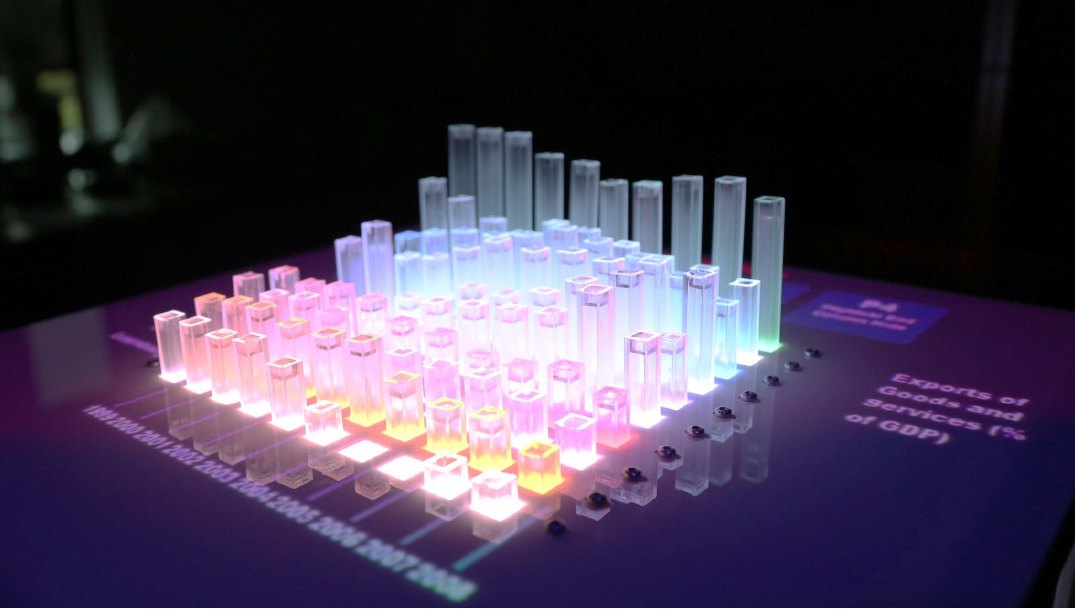
\includegraphics[width=0.5\textwidth]{img/taher2015-emerge.png} 
\caption{EMERGE: Exploring Interactions with Physically Dynamic Bar Charts using actuating physical rods and RGB LEDs to display international export data.}\label{fig:taher2015-emerge}
\end{figure}

EMERGE allows users to interact with the dataset it represents using a set of 4 interaction-sets derived from subcategories of the taxonomy of interactive dynamics for visual analysis described by \citet{heer2012} - \textit{annotation}, \textit{filtering}, \textit{organisation} and \textit{navigation} (Table \ref{tbl:taher2015-user-study}).  \citeauthor{heer2012} lay out 3 high-level categories in their model - \textit{Data and View Specification}, \textit{View Manipulation}, and \textit{Process and Provenance}. (Figure \ref{fig:heer2012-taxonomy}). In this sense, whilst the selection of InfoVis model is careful and grounded in background theory, the choice of subcategories by \citeauthor{taher2015} for interacting with EMERGE is somewhat arbitrary and limited in scope with little justification, which immediately invites further research into different forms of interactions with physicalisations from the taxonomy.

\begin{table}[H]
\centering
\caption{Task-sets and interaction techniques explored during the user study with EMERGE: \textit{annotation}, \textit{filtering}, \textit{organisation} and \textit{navigation} with the category of \protect\citet{heer2012} in \textbf{bold}.}\label{tbl:taher2015-user-study}
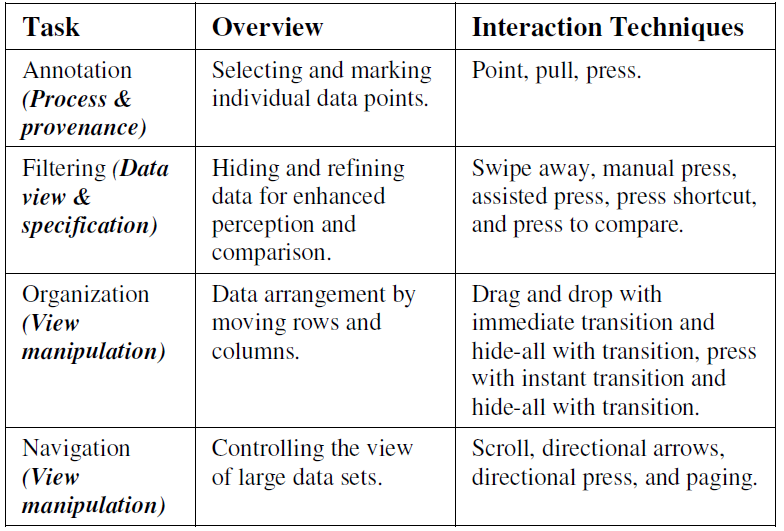
\includegraphics[width=0.65\textwidth]{img/taher2015-user-study.png} 
\end{table}

\begin{figure}[H]
\centering
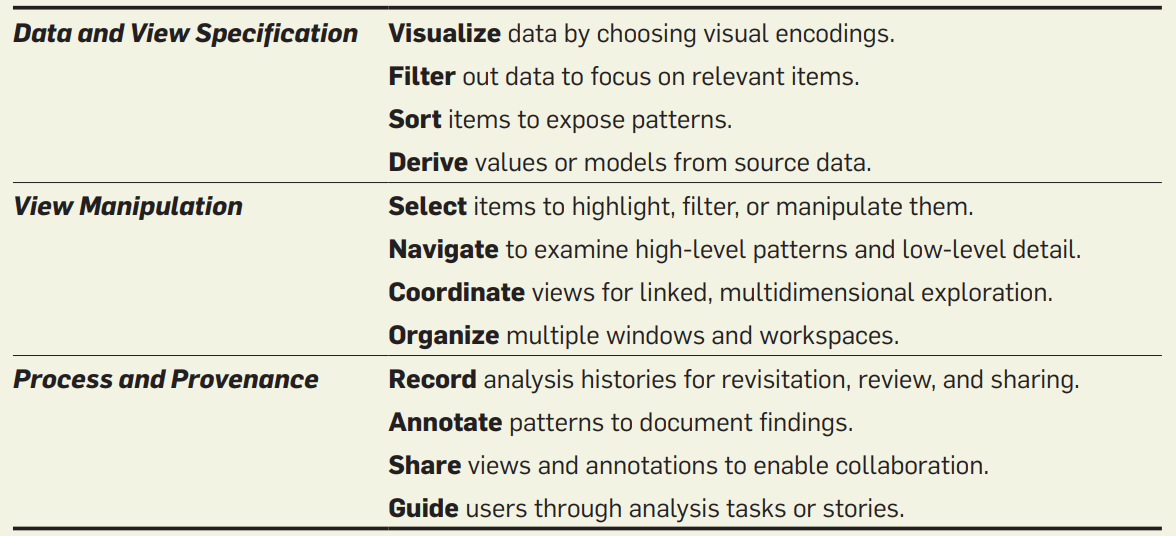
\includegraphics[width=0.8\textwidth]{img/heer2012-taxonomy.png} 
\caption{Taxonomy of interactive dynamics described by \protect\citet{heer2012}.}\label{fig:heer2012-taxonomy}
\end{figure}

Main contributions of \citet{taher2015} are threefold. First, a set of 14 potential interactions (both physical and gesture based) for manipulating and exploring data presented in dynamic physical bar charts such as EMERGE. Second, the findings of their user study ($N=17$) evaluates which of the interactions are effective and intuitive in completing a set of analysis tasks, and which interactions match users' initial preconceptions for how to achieve these tasks. Finally, a set of design considerations to advise future research on the challenges of presenting data in physically dynamic form. Overall, we learn that a \textit{combination} of gestures and physical interactions are effective. Smaller interactions such as annotation of specific data points can be afforded by physical interaction whereas larger interactions such as organization can be afforded touch-screen gestures. 

\sectiontitle{Justifications for Conclusions}
\citeauthor{taher2015} set about their investigations by creating a list of proposed or \textit{baseline} interactions by which users could interact with EMERGE. The authors by their own admission avoided early experimentation to generate different types of interaction before the main study as existing research forewarned against this due to the immaturity of the area \citep{hornbaek2013}. Whilst this was sensible to consider, the mechanics of the baseline interactions to be used in the user study are strongly-coupled with the hardware capabilities of EMERGE and no explanation is given by the authors into where the inspiration for each proposed interaction came from, which causes some early concern over generalisability of results to other implementations of physically dynamic bar charts.

A user study ($N=17$, 6 female) involved 

\begin{figure}[H]
\minipage{0.5\textwidth}
\centering
  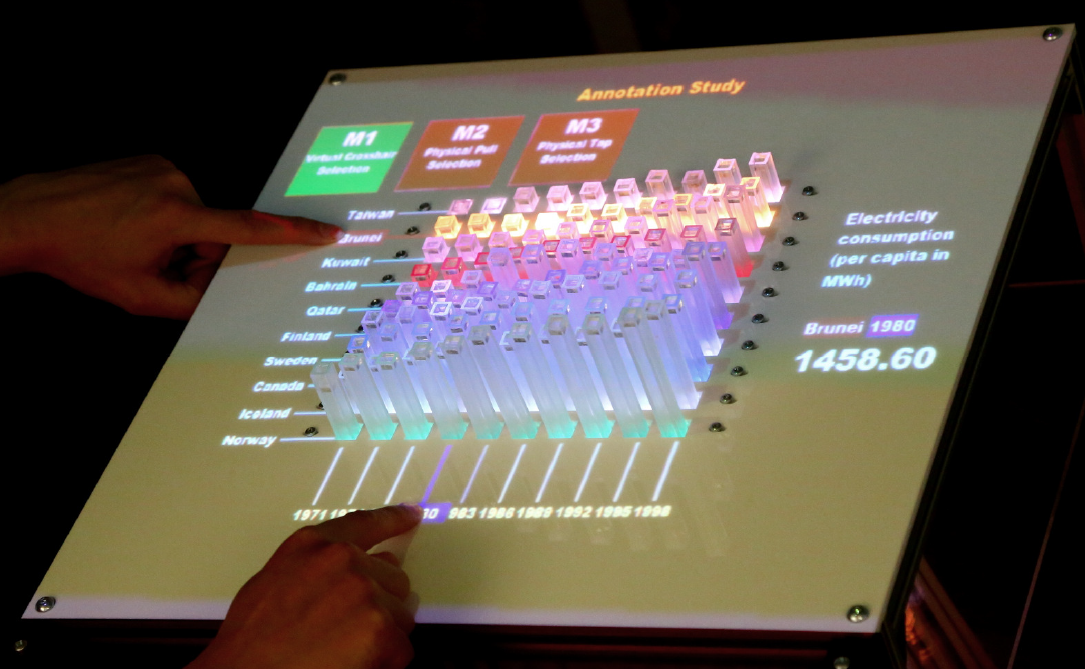
\includegraphics[height=3.5cm]{img/taher2015-annotation.png}
  \caption{Annotation (Point technique).}\label{fig:taher2015-annotation}
\endminipage\hfill
\minipage{0.5\textwidth}%
\centering
  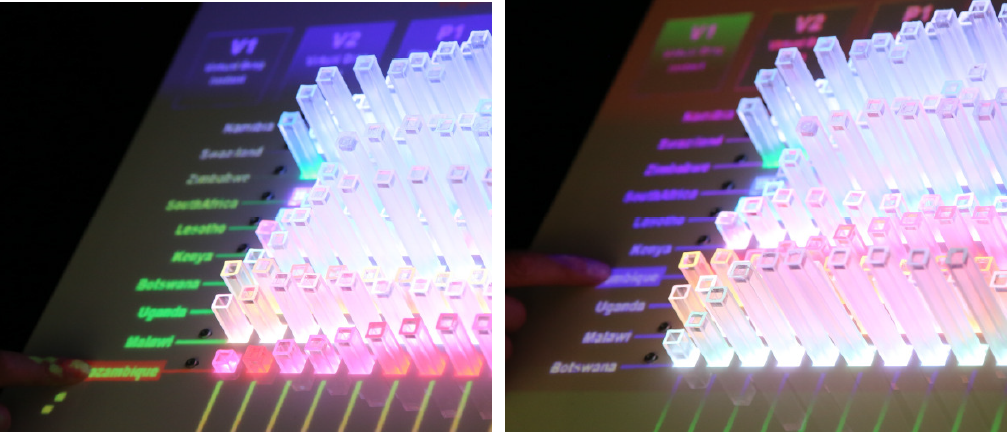
\includegraphics[height=3.5cm]{img/taher2015-organize.png}
  \caption{Organisation (Drag and Drop technique).}\label{fig:taher2015-organize}
\endminipage
\end{figure}

\begin{figure}[H]
\centering
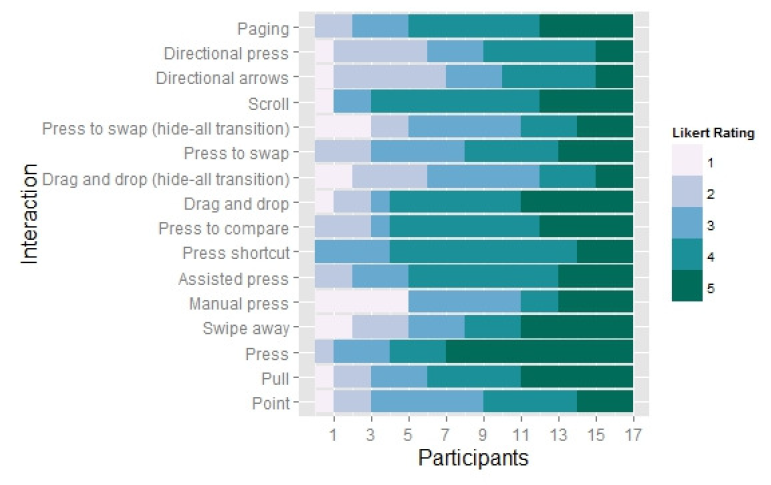
\includegraphics[width=0.5\textwidth]{img/taher2015-likert.png} 
\caption{Likert scale ratings for helpfulness of interaction
techniques. Range = 1: Strongly Disagree, 5: Strongly Agree.}\label{fig:taher2015-likert}
\end{figure}

\sectiontitle{Limitations and Suggested Further Work}
\citet{taher2015} present a respectable investigation of potential techniques to interact with data presented in a physically dynamic form and their conclusion on the usefulness of both physical and gesture-based interactions with these systems seems valid, but a set of limitations with their work leads to some questions being open to future research. 

Crucially, the number of participants involved should be increased and to ensure conclusions are generalisable with external validity, the sample should be representative of the general population (approx. $50\%$ gender split). Also, aside from the Likert scale data, the paper lacks a lot of parametric data which might provide further insight into efficacy of interactions - further controlled studies could attempt to measure performance metrics such as task completion times and accuracy for each interaction type.

Seeing as the investigation focuses on a narrow subset of the interaction taxonomy of \citet{heer2012} on a Bar Chart, the obvious extensions to the authors' work would be to explore different interaction types such as Record, Co-ordinate and Share using EMERGE, and extend experiments across different point systems such as Dynamic Histograms, Parallel Coordinates and Theme Rivers. Seeing as the conclusion of the paper is that \textit{both} physical and gesture based interactions are effective for small and large grained tasks respectively, it would be wise to see how \textit{combining} both interactions into one activity affects findings.

The authors concede themselves that the hardware implementation of EMERGE presents a large limitation in their findings. Firstly, the chart itself is of a 3D modality with no vertical axis. The only meaningful vertical information is ascertained by visual comparison of bar heights rather than reading of direct data. Secondly, the representation of larger datasets would require a far more data points than the $10\times10$ grid currently allows for - it is likely that for higher resolution of data points, navigation interactions such as pagination would suffice whereas pressing data points to navigate between single rows would be cumbersome. Thirdly, the technical challenges discussed previously (actuation speed and noise, rod spacing, size of setup) may have also mediated or impacted the results in ways that were not accounted for. Almost all participants reacted hesitantly due to these speed and noise of actuation. Further analysis (e.g. use of parallel mediated regression testing) should investigate this.

The InfoVis design space is very large \citep{card1997}, so it would be novel to explore how users perceive dynamic physicalisations which represent complex datasets which \textit{change} in real time - e.g. social network data \citep{federico2011}. As well as responding to human interaction via shape-changing interfaces, these datasets could also change of their own accord which opens up more questions into how users would respond to this type of visualisation. Another novel suggestion would be to apply these visualisations to a specific context or domain, to compare efficacy of interactions across modalities (i.e. \textit{static physical} versus \textit{dynamic physical} versus \textit{virtual}). An example might be in an educational setting where kinaesthetic techniques are encouraged \citep{gilakjani2011}. Furthermore, investigations could also be extended to observe the effects of using dynamic physicalisations whilst a user is immersed in a VR environment, to combat a lack of `presence' in these settings and afford data manipulation in virtual settings with physical assistance \citep{tennent2017}.

\sectiontitle{Conclusion}
\citet{taher2015} set the foundations for future investigations into use of shape-changing displays for accomplishment of common InfoVis tasks. Their research is limited in several ways by the implementation of the EMERGE system, but raises important design considerations for future work investigating dynamic physicalisations in other domains. Findings have potentially wider consequences in the topic of Information Visualisation - with recommendations on how to design systems supporting the fundamental interactions such as those described by \citet{heer2012}, these visualisations can serve as effective data analysis tools in a variety of domains.

\wordcount{1289}

\newpage
\small
\bibliography{bib2}
\normalsize
\end{document}